\documentclass[a4paper]{article}

\def\npart{III}
\def\nterm {Lent}
\def\nyear {2017-2018}
\def\nlecturer {Brian}
\def\ncourse {Mechanics}

\makeatletter
\ifx \nauthor\undefined
  \def\nauthor{Dexter Chua}
\else
\fi

\author{Based on lectures by \nlecturer \\\small Notes taken by \nauthor}
\date{\nterm\ \nyear}

\usepackage{alltt}
\usepackage{amsfonts}
\usepackage{amsmath}
\usepackage{amssymb}
\usepackage{amsthm}
\usepackage{booktabs}
\usepackage{caption}
\usepackage{enumitem}
\usepackage{fancyhdr}
\usepackage{graphicx}
\usepackage{mathdots}
\usepackage{mathtools}
\usepackage{microtype}
\usepackage{multirow}
\usepackage{pdflscape}
\usepackage{pgfplots}
\usepackage{siunitx}
\usepackage{slashed}
\usepackage{tabularx}
\usepackage{tikz}
\usepackage{tkz-euclide}
\usepackage[normalem]{ulem}
\usepackage[all]{xy}
\usepackage{imakeidx}

\makeindex[intoc, title=Index]
\indexsetup{othercode={\lhead{\emph{Index}}}}

\ifx \nextra \undefined
  \usepackage[pdftex,
    hidelinks,
    pdfauthor={Dexter Chua},
    pdfsubject={Cambridge Maths Notes: Part \npart\ - \ncourse},
    pdftitle={Part \npart\ - \ncourse},
  pdfkeywords={Cambridge Mathematics Maths Math \npart\ \nterm\ \nyear\ \ncourse}]{hyperref}
  \title{Part \npart\ --- \ncourse}
\else
  \usepackage[pdftex,
    hidelinks,
    pdfauthor={Dexter Chua},
    pdfsubject={Cambridge Maths Notes: Part \npart\ - \ncourse\ (\nextra)},
    pdftitle={Part \npart\ - \ncourse\ (\nextra)},
  pdfkeywords={Cambridge Mathematics Maths Math \npart\ \nterm\ \nyear\ \ncourse\ \nextra}]{hyperref}

  \title{Part \npart\ --- \ncourse \\ {\Large \nextra}}
  \renewcommand\printindex{}
\fi

\pgfplotsset{compat=1.12}

\pagestyle{fancyplain}
\ifx \ncoursehead \undefined
\def\ncoursehead{\ncourse}
\fi

\lhead{\emph{\nouppercase{\leftmark}}}
\ifx \nextra \undefined
  \rhead{
    \ifnum\thepage=1
    \else
      \npart\ \ncoursehead
    \fi}
\else
  \rhead{
    \ifnum\thepage=1
    \else
      \npart\ \ncoursehead \ (\nextra)
    \fi}
\fi
\usetikzlibrary{arrows.meta}
\usetikzlibrary{decorations.markings}
\usetikzlibrary{decorations.pathmorphing}
\usetikzlibrary{positioning}
\usetikzlibrary{fadings}
\usetikzlibrary{intersections}
\usetikzlibrary{cd}

\newcommand*{\Cdot}{{\raisebox{-0.25ex}{\scalebox{1.5}{$\cdot$}}}}
\newcommand {\pd}[2][ ]{
  \ifx #1 { }
    \frac{\partial}{\partial #2}
  \else
    \frac{\partial^{#1}}{\partial #2^{#1}}
  \fi
}
\ifx \nhtml \undefined
\else
  \renewcommand\printindex{}
  \DisableLigatures[f]{family = *}
  \let\Contentsline\contentsline
  \renewcommand\contentsline[3]{\Contentsline{#1}{#2}{}}
  \renewcommand{\@dotsep}{10000}
  \newlength\currentparindent
  \setlength\currentparindent\parindent

  \newcommand\@minipagerestore{\setlength{\parindent}{\currentparindent}}
  \usepackage[active,tightpage,pdftex]{preview}
  \renewcommand{\PreviewBorder}{0.1cm}

  \newenvironment{stretchpage}%
  {\begin{preview}\begin{minipage}{\hsize}}%
    {\end{minipage}\end{preview}}
  \AtBeginDocument{\begin{stretchpage}}
  \AtEndDocument{\end{stretchpage}}

  \newcommand{\@@newpage}{\end{stretchpage}\begin{stretchpage}}

  \let\@real@section\section
  \renewcommand{\section}{\@@newpage\@real@section}
  \let\@real@subsection\subsection
  \renewcommand{\subsection}{\@ifstar{\@real@subsection*}{\@@newpage\@real@subsection}}
\fi
\ifx \ntrim \undefined
\else
  \usepackage{geometry}
  \geometry{
    papersize={379pt, 699pt},
    textwidth=345pt,
    textheight=596pt,
    left=17pt,
    top=54pt,
    right=17pt
  }
\fi

\ifx \nisofficial \undefined
\let\@real@maketitle\maketitle
\renewcommand{\maketitle}{\@real@maketitle\begin{center}\begin{minipage}[c]{0.9\textwidth}\centering\footnotesize These notes are not endorsed by the lecturers, and I have modified them (often significantly) after lectures. They are nowhere near accurate representations of what was actually lectured, and in particular, all errors are almost surely mine.\end{minipage}\end{center}}
\else
\fi

% Theorems
\theoremstyle{definition}
\newtheorem*{aim}{Aim}
\newtheorem*{axiom}{Axiom}
\newtheorem*{claim}{Claim}
\newtheorem*{cor}{Corollary}
\newtheorem*{conjecture}{Conjecture}
\newtheorem*{defi}{Definition}
\newtheorem*{eg}{Example}
\newtheorem*{ex}{Exercise}
\newtheorem*{fact}{Fact}
\newtheorem*{law}{Law}
\newtheorem*{lemma}{Lemma}
\newtheorem*{notation}{Notation}
\newtheorem*{prop}{Proposition}
\newtheorem*{question}{Question}
\newtheorem*{rrule}{Rule}
\newtheorem*{thm}{Theorem}
\newtheorem*{assumption}{Assumption}

\newtheorem*{remark}{Remark}
\newtheorem*{warning}{Warning}
\newtheorem*{exercise}{Exercise}

\newtheorem{nthm}{Theorem}[section]
\newtheorem{nlemma}[nthm]{Lemma}
\newtheorem{nprop}[nthm]{Proposition}
\newtheorem{ncor}[nthm]{Corollary}


\renewcommand{\labelitemi}{--}
\renewcommand{\labelitemii}{$\circ$}
\renewcommand{\labelenumi}{(\roman{*})}

\let\stdsection\section
\renewcommand\section{\newpage\stdsection}

\newcommand\qedsym{\hfill\ensuremath{\square}}
% Strike through
\def\st{\bgroup \ULdepth=-.55ex \ULset}


%%%%%%%%%%%%%%%%%%%%%%%%%
%%%%% Maths Symbols %%%%%
%%%%%%%%%%%%%%%%%%%%%%%%%

% Matrix groups
\newcommand{\GL}{\mathrm{GL}}
\newcommand{\Or}{\mathrm{O}}
\newcommand{\PGL}{\mathrm{PGL}}
\newcommand{\PSL}{\mathrm{PSL}}
\newcommand{\PSO}{\mathrm{PSO}}
\newcommand{\PSU}{\mathrm{PSU}}
\newcommand{\SL}{\mathrm{SL}}
\newcommand{\SO}{\mathrm{SO}}
\newcommand{\Spin}{\mathrm{Spin}}
\newcommand{\Sp}{\mathrm{Sp}}
\newcommand{\SU}{\mathrm{SU}}
\newcommand{\U}{\mathrm{U}}
\newcommand{\Mat}{\mathrm{Mat}}

% Matrix algebras
\newcommand{\gl}{\mathfrak{gl}}
\newcommand{\ort}{\mathfrak{o}}
\newcommand{\so}{\mathfrak{so}}
\newcommand{\su}{\mathfrak{su}}
\newcommand{\uu}{\mathfrak{u}}
\renewcommand{\sl}{\mathfrak{sl}}

% Special sets
\newcommand{\C}{\mathbb{C}}
\newcommand{\CP}{\mathbb{CP}}
\newcommand{\GG}{\mathbb{G}}
\newcommand{\N}{\mathbb{N}}
\newcommand{\Q}{\mathbb{Q}}
\newcommand{\R}{\mathbb{R}}
\newcommand{\RP}{\mathbb{RP}}
\newcommand{\T}{\mathbb{T}}
\newcommand{\Z}{\mathbb{Z}}
\renewcommand{\H}{\mathbb{H}}

% Brackets
\newcommand{\abs}[1]{\left\lvert #1\right\rvert}
\newcommand{\bket}[1]{\left\lvert #1\right\rangle}
\newcommand{\brak}[1]{\left\langle #1 \right\rvert}
\newcommand{\braket}[2]{\left\langle #1\middle\vert #2 \right\rangle}
\newcommand{\bra}{\langle}
\newcommand{\ket}{\rangle}
\newcommand{\norm}[1]{\left\lVert #1\right\rVert}
\newcommand{\normalorder}[1]{\mathop{:}\nolimits\!#1\!\mathop{:}\nolimits}
\newcommand{\tv}[1]{|#1|}
\renewcommand{\vec}[1]{\boldsymbol{\mathbf{#1}}}

% not-math
\newcommand{\bolds}[1]{{\bfseries #1}}
\newcommand{\cat}[1]{\mathsf{#1}}
\newcommand{\ph}{\,\cdot\,}
\newcommand{\term}[1]{\emph{#1}\index{#1}}
\newcommand{\phantomeq}{\hphantom{{}={}}}
% Probability
\DeclareMathOperator{\Bernoulli}{Bernoulli}
\DeclareMathOperator{\betaD}{beta}
\DeclareMathOperator{\bias}{bias}
\DeclareMathOperator{\binomial}{binomial}
\DeclareMathOperator{\corr}{corr}
\DeclareMathOperator{\cov}{cov}
\DeclareMathOperator{\gammaD}{gamma}
\DeclareMathOperator{\mse}{mse}
\DeclareMathOperator{\multinomial}{multinomial}
\DeclareMathOperator{\Poisson}{Poisson}
\DeclareMathOperator{\var}{var}
\newcommand{\E}{\mathbb{E}}
\newcommand{\Prob}{\mathbb{P}}

% Algebra
\DeclareMathOperator{\adj}{adj}
\DeclareMathOperator{\Ann}{Ann}
\DeclareMathOperator{\Aut}{Aut}
\DeclareMathOperator{\Char}{char}
\DeclareMathOperator{\disc}{disc}
\DeclareMathOperator{\dom}{dom}
\DeclareMathOperator{\fix}{fix}
\DeclareMathOperator{\Hom}{Hom}
\DeclareMathOperator{\id}{id}
\DeclareMathOperator{\image}{image}
\DeclareMathOperator{\im}{im}
\DeclareMathOperator{\tr}{tr}
\DeclareMathOperator{\Tr}{Tr}
\newcommand{\Bilin}{\mathrm{Bilin}}
\newcommand{\Frob}{\mathrm{Frob}}

% Others
\newcommand\ad{\mathrm{ad}}
\newcommand\Art{\mathrm{Art}}
\newcommand{\B}{\mathcal{B}}
\newcommand{\cU}{\mathcal{U}}
\newcommand{\Der}{\mathrm{Der}}
\newcommand{\D}{\mathrm{D}}
\newcommand{\dR}{\mathrm{dR}}
\newcommand{\exterior}{\mathchoice{{\textstyle\bigwedge}}{{\bigwedge}}{{\textstyle\wedge}}{{\scriptstyle\wedge}}}
\newcommand{\F}{\mathbb{F}}
\newcommand{\G}{\mathcal{G}}
\newcommand{\Gr}{\mathrm{Gr}}
\newcommand{\haut}{\mathrm{ht}}
\newcommand{\Hol}{\mathrm{Hol}}
\newcommand{\hol}{\mathfrak{hol}}
\newcommand{\Id}{\mathrm{Id}}
\newcommand{\lie}[1]{\mathfrak{#1}}
\newcommand{\op}{\mathrm{op}}
\newcommand{\Oc}{\mathcal{O}}
\newcommand{\pr}{\mathrm{pr}}
\newcommand{\Ps}{\mathcal{P}}
\newcommand{\pt}{\mathrm{pt}}
\newcommand{\qeq}{\mathrel{``{=}"}}
\newcommand{\Rs}{\mathcal{R}}
\newcommand{\Vect}{\mathrm{Vect}}
\newcommand{\wsto}{\stackrel{\mathrm{w}^*}{\to}}
\newcommand{\wt}{\mathrm{wt}}
\newcommand{\wto}{\stackrel{\mathrm{w}}{\to}}
\renewcommand{\d}{\mathrm{d}}
\renewcommand{\P}{\mathbb{P}}
%\renewcommand{\F}{\mathcal{F}}


\let\Im\relax
\let\Re\relax

\DeclareMathOperator{\area}{area}
\DeclareMathOperator{\card}{card}
\DeclareMathOperator{\ccl}{ccl}
\DeclareMathOperator{\ch}{ch}
\DeclareMathOperator{\cl}{cl}
\DeclareMathOperator{\cls}{\overline{\mathrm{span}}}
\DeclareMathOperator{\coker}{coker}
\DeclareMathOperator{\conv}{conv}
\DeclareMathOperator{\cosec}{cosec}
\DeclareMathOperator{\cosech}{cosech}
\DeclareMathOperator{\covol}{covol}
\DeclareMathOperator{\diag}{diag}
\DeclareMathOperator{\diam}{diam}
\DeclareMathOperator{\Diff}{Diff}
\DeclareMathOperator{\End}{End}
\DeclareMathOperator{\energy}{energy}
\DeclareMathOperator{\erfc}{erfc}
\DeclareMathOperator{\erf}{erf}
\DeclareMathOperator*{\esssup}{ess\,sup}
\DeclareMathOperator{\ev}{ev}
\DeclareMathOperator{\Ext}{Ext}
\DeclareMathOperator{\fst}{fst}
\DeclareMathOperator{\Fit}{Fit}
\DeclareMathOperator{\Frac}{Frac}
\DeclareMathOperator{\Gal}{Gal}
\DeclareMathOperator{\gr}{gr}
\DeclareMathOperator{\hcf}{hcf}
\DeclareMathOperator{\Im}{Im}
\DeclareMathOperator{\Ind}{Ind}
\DeclareMathOperator{\Int}{Int}
\DeclareMathOperator{\Isom}{Isom}
\DeclareMathOperator{\lcm}{lcm}
\DeclareMathOperator{\length}{length}
\DeclareMathOperator{\Lie}{Lie}
\DeclareMathOperator{\like}{like}
\DeclareMathOperator{\Lk}{Lk}
\DeclareMathOperator{\Maps}{Maps}
\DeclareMathOperator{\orb}{orb}
\DeclareMathOperator{\ord}{ord}
\DeclareMathOperator{\otp}{otp}
\DeclareMathOperator{\poly}{poly}
\DeclareMathOperator{\rank}{rank}
\DeclareMathOperator{\rel}{rel}
\DeclareMathOperator{\Rad}{Rad}
\DeclareMathOperator{\Re}{Re}
\DeclareMathOperator*{\res}{res}
\DeclareMathOperator{\Res}{Res}
\DeclareMathOperator{\Ric}{Ric}
\DeclareMathOperator{\rk}{rk}
\DeclareMathOperator{\Rees}{Rees}
\DeclareMathOperator{\Root}{Root}
\DeclareMathOperator{\sech}{sech}
\DeclareMathOperator{\sgn}{sgn}
\DeclareMathOperator{\snd}{snd}
\DeclareMathOperator{\Spec}{Spec}
\DeclareMathOperator{\spn}{span}
\DeclareMathOperator{\stab}{stab}
\DeclareMathOperator{\St}{St}
\DeclareMathOperator{\supp}{supp}
\DeclareMathOperator{\Syl}{Syl}
\DeclareMathOperator{\Sym}{Sym}
\DeclareMathOperator{\vol}{vol}

\pgfarrowsdeclarecombine{twolatex'}{twolatex'}{latex'}{latex'}{latex'}{latex'}
\tikzset{->/.style = {decoration={markings,
                                  mark=at position 1 with {\arrow[scale=2]{latex'}}},
                      postaction={decorate}}}
\tikzset{<-/.style = {decoration={markings,
                                  mark=at position 0 with {\arrowreversed[scale=2]{latex'}}},
                      postaction={decorate}}}
\tikzset{<->/.style = {decoration={markings,
                                   mark=at position 0 with {\arrowreversed[scale=2]{latex'}},
                                   mark=at position 1 with {\arrow[scale=2]{latex'}}},
                       postaction={decorate}}}
\tikzset{->-/.style = {decoration={markings,
                                   mark=at position #1 with {\arrow[scale=2]{latex'}}},
                       postaction={decorate}}}
\tikzset{-<-/.style = {decoration={markings,
                                   mark=at position #1 with {\arrowreversed[scale=2]{latex'}}},
                       postaction={decorate}}}
\tikzset{->>/.style = {decoration={markings,
                                  mark=at position 1 with {\arrow[scale=2]{latex'}}},
                      postaction={decorate}}}
\tikzset{<<-/.style = {decoration={markings,
                                  mark=at position 0 with {\arrowreversed[scale=2]{twolatex'}}},
                      postaction={decorate}}}
\tikzset{<<->>/.style = {decoration={markings,
                                   mark=at position 0 with {\arrowreversed[scale=2]{twolatex'}},
                                   mark=at position 1 with {\arrow[scale=2]{twolatex'}}},
                       postaction={decorate}}}
\tikzset{->>-/.style = {decoration={markings,
                                   mark=at position #1 with {\arrow[scale=2]{twolatex'}}},
                       postaction={decorate}}}
\tikzset{-<<-/.style = {decoration={markings,
                                   mark=at position #1 with {\arrowreversed[scale=2]{twolatex'}}},
                       postaction={decorate}}}

\tikzset{circ/.style = {fill, circle, inner sep = 0, minimum size = 3}}
\tikzset{scirc/.style = {fill, circle, inner sep = 0, minimum size = 1.5}}
\tikzset{mstate/.style={circle, draw, blue, text=black, minimum width=0.7cm}}

\tikzset{eqpic/.style={baseline={([yshift=-.5ex]current bounding box.center)}}}
\tikzset{commutative diagrams/.cd,cdmap/.style={/tikz/column 1/.append style={anchor=base east},/tikz/column 2/.append style={anchor=base west},row sep=tiny}}

\definecolor{mblue}{rgb}{0.2, 0.3, 0.8}
\definecolor{morange}{rgb}{1, 0.5, 0}
\definecolor{mgreen}{rgb}{0.1, 0.4, 0.2}
\definecolor{mred}{rgb}{0.5, 0, 0}

\def\drawcirculararc(#1,#2)(#3,#4)(#5,#6){%
    \pgfmathsetmacro\cA{(#1*#1+#2*#2-#3*#3-#4*#4)/2}%
    \pgfmathsetmacro\cB{(#1*#1+#2*#2-#5*#5-#6*#6)/2}%
    \pgfmathsetmacro\cy{(\cB*(#1-#3)-\cA*(#1-#5))/%
                        ((#2-#6)*(#1-#3)-(#2-#4)*(#1-#5))}%
    \pgfmathsetmacro\cx{(\cA-\cy*(#2-#4))/(#1-#3)}%
    \pgfmathsetmacro\cr{sqrt((#1-\cx)*(#1-\cx)+(#2-\cy)*(#2-\cy))}%
    \pgfmathsetmacro\cA{atan2(#2-\cy,#1-\cx)}%
    \pgfmathsetmacro\cB{atan2(#6-\cy,#5-\cx)}%
    \pgfmathparse{\cB<\cA}%
    \ifnum\pgfmathresult=1
        \pgfmathsetmacro\cB{\cB+360}%
    \fi
    \draw (#1,#2) arc (\cA:\cB:\cr);%
}
\newcommand\getCoord[3]{\newdimen{#1}\newdimen{#2}\pgfextractx{#1}{\pgfpointanchor{#3}{center}}\pgfextracty{#2}{\pgfpointanchor{#3}{center}}}

\newcommand\qedshift{\vspace{-17pt}}
\newcommand\fakeqed{\pushQED{\qed}\qedhere}

\def\Xint#1{\mathchoice
   {\XXint\displaystyle\textstyle{#1}}%
   {\XXint\textstyle\scriptstyle{#1}}%
   {\XXint\scriptstyle\scriptscriptstyle{#1}}%
   {\XXint\scriptscriptstyle\scriptscriptstyle{#1}}%
   \!\int}
\def\XXint#1#2#3{{\setbox0=\hbox{$#1{#2#3}{\int}$}
     \vcenter{\hbox{$#2#3$}}\kern-.5\wd0}}
\def\ddashint{\Xint=}
\def\dashint{\Xint-}

\newcommand\separator{{\centering\rule{2cm}{0.2pt}\vspace{2pt}\par}}

\newenvironment{own}{\color{gray!70!black}}{}

\newcommand\makecenter[1]{\raisebox{-0.5\height}{#1}}

\mathchardef\mdash="2D

\newenvironment{significant}{\begin{center}\begin{minipage}{0.9\textwidth}\centering\em}{\end{minipage}\end{center}}
\DeclareRobustCommand{\rvdots}{%
  \vbox{
    \baselineskip4\p@\lineskiplimit\z@
    \kern-\p@
    \hbox{.}\hbox{.}\hbox{.}
  }}
\DeclareRobustCommand\tph[3]{{\texorpdfstring{#1}{#2}}}
\makeatother


\begin{document}

\maketitle


\tableofcontents

\section{Kinematics of a particles moving in a straight line}

\section{Dynamics of a particle moving in a straight line}

\section{Statics of a particle}

\section{Moments}

\section{Vectors}

\section{Kinematics of a particle moving in a straight line or plane}

\section{Centres of mass}

\section{Work , energy and power}

\section{Collisions}

\section{Statics of rigid bodies 1}

\section{Further kinematics}
\subsection{Forces which vary with speed}
\begin{prop}
	\[
		\mathbf{a}=\mathbf{v}\frac{\d \mathbf{v}}{\d \mathbf{x}}
	\]
	\begin{proof}
		\[
			\mathbf{a}=\frac{\d \mathbf{x}}{\d \mathbf{t}}\times \frac{\d \mathbf{v}}{\d \mathbf{x}}=\mathbf{v}\frac{\d \mathbf{v}}{\d \mathbf{x}}
		\]
	\end{proof}
\end{prop}
\section{Elastic strings and springs}
\subsection{Hooke's Law}
\begin{law}[Hooke's Law]
	There are two cases for using Hooke's Law
	\begin{enumerate}
		\item Elastic strings: The tension $T$ in an elastic string is
		      \[
			      T=\frac{\lambda x}{l}
		      \]
		      where \\
		      $l$ is the natural (unstretched) length of the string,\\
		      $x$ is the extension and\\
		      $\lambda$ is the modulus of elasticity
		      \begin{center}
			      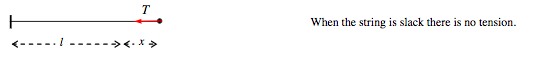
\includegraphics[scale=0.5]{img_M/12_intro1}
		      \end{center}
		\item Elastic springs: The tension, or thrust, $T$ is an elastic spring is
		      \[
			      T=\frac{\lambda x}{l}
		      \]
		      where \\
		      $l$ is the natural (unstretched) length of the string,\\
		      $x$ is the extension or compression and\\
		      $\lambda$ is the modulus of elasticity
		      \begin{center}
			      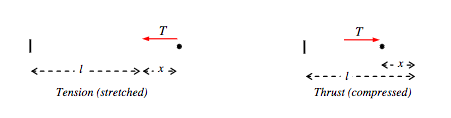
\includegraphics[scale=0.5]{img_M/12_intro2}
		      \end{center}
	\end{enumerate}
\end{law}

\subsection{Energy stored in an elastic string or spring}
Like kinematics,If there is force $F$ and displacement traveled $\delta s$, the Work done is $\delta W=F\delta s$. Similarly, If the tension force is $T$ and string/spring extended/stretched, then
\[
	\delta W \approx T \delta x
\]
Total work done in exrending from $x=0$ to $x=X$ is approximately
\[
	\sum^{X}_0 T \delta x
\]

and , as $\delta x \rightarrow 0 $, the total work done:

\[
	W=\int^X_0 T \d x= \int^X_0 \frac{\lambda x}{l}\d x=\frac{\lambda x^2}{2l}
\]
The expression of Total work done is also called the Elastic Potential Energy

\section{Further dynamics}
\subsection{Impulse of a variable force}
\[
	\delta I \approx F(t) \delta t
\]
The total impulse from time $t_1$ to $t_2$ is
\[
	I \approx \sum_{t_1}^{t_2} F(t) \delta t
\]
and as $\delta t \rightarrow 0$, the total impulse is
\[
	I=\int^{t_2}_{t_1} F(t) \d t
\]
Also, as $F(t)=ma=m\frac{\d v}{\d t}$
\begin{align*}
	\int_{t_1}^{t_2} F(t) \d t & =\int^{V}_{U} m \d v =mV-mU
\end{align*}
\subsection{Work done by a variable force}
\[
	\delta W \approx G(x)\delta x
\]
and the total work done in moving from a displacement $x_1$ to $x_2$ is
\[
	W\approx\sum_{x_1}^{x_2} G(x)\delta x
\]
and as $\delta x \rightarrow 0$ , the total work done is
\[
	W=\int_{x_1}^{x_2} G(x) \d x
\]
Also $G(x)=ma=m\frac{\d v}{\d x}=m\frac{\d x}{\d t}\times \frac{\d v}{\d x}=mv\frac{\d v}{\d x}$
\[
	\int_{x_1}^{x_2} G(x) \d x =\int_U^V mv \d v =\frac{1}{2}mV^2-\frac{1}{2}mU^2
\]

\subsection{Newton's Law of Gravitation}
\begin{law}
	The force of attraction between two bodies of masses
	$M_1$
	and
	$M_2$
	is directly proportional to the product of their masses and inversely proportional to the square of the distance,
	$d$ , between them:
	\[
		F=\frac{GM_1M_2}{d^2}
	\]
	where $G$ is a constant known as the constant of Gravitation
\end{law}
\subsection{Finding $k$ in $F=\frac{k}{x^2}$}
\[
	F=ma=\frac{k}{d^2}
\]

\subsection{Simple harmonic motion S.H.M.}

\begin{defi}[S.H.M. equation]
	If a particle
	,
	$P$
	, moves in a straight line so that
	its acceleration is proportional to its distance
	from a fixed point
	$O$
	, and directed towards
	$O$
	,
	then
	\[
		\ddot{x}=-\omega^2x
	\]
	and the particle will oscillate between two points,
	$A$
	and
	$B$
	, with simple harmonic motion.\\

	The amplitude of the oscillation is
	$OA = OB= a$.\\

	Notice that $\ddot{x}$
	is marked
	in the direction of
	$x$
	increasing
	$n$ the diagram
	, and, since
	$\omega^2$
	is
	positive,
	$\ddot{x}$
	is negative
	, so the acceleration acts towards
	$O$.
	\begin{center}
		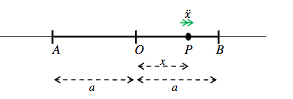
\includegraphics[scale=0.5]{img_M/12_intro4}
	\end{center}
\end{defi}

\begin{prop}[Solving equation]
	A.E. is
	\[
		m^2=-\omega^2 \rightarrow m=i\omega
	\]
	G.S. is
	\[
		x=\lambda \sin \omega t+\mu \cos \omega t
	\]
	If $x$ starts from $O$, $x=O$ when $t=0$, \\
	then
	\[
		x=a \sin\omega t
	\]
	If $x$ starts from $B$, $x=a$ when $t=0$, \\
	then
	\[
		x=a\cos\omega t
	\]
\end{prop}
\begin{defi}[Period and amplitude]
	From the equations $x=a \sin\omega t$ and $x=a\cos\omega t$\\
	we can see that the period, the time for one complete oscillation, is
	\[
		T=\frac{2\pi}{\omega}
	\]
	The period is the time taken to go from $O\rightarrow B\rightarrow A\rightarrow O$, or from $B\rightarrow A \rightarrow B$ and that the
	amplitude, maximum distance from the central point, is $a$.
\end{defi}

\begin{prop}[Alternative equation of S.H.M.]
	\[
		v^2=\omega^2(a^2-x^2)
	\]
	\begin{proof}
		Consider the basic S.H.M. equation $\ddot{x}=-\omega^2x$ and $\ddot{x}=v \frac{\d v}{\d x}$
		\begin{align*}
			v \frac{\d v}{\d x} & =-\omega^2x                           \\
			\int v \d v         & =\int -\omega^2 x \d x                \\
			\frac{1}{2}v^2      & =-\frac{1}{2}\omega^2x^2+\frac{1}{2}c
		\end{align*}
		But $v=)$ when $x$ at its maxumum, $x= a \rightarrow c=a^2\omega^2$
		\begin{align*}
			\frac{1}{2}v^2 & =-\frac{1}{2}\omega^2x^2+\frac{1}{2}a^2\omega^2 \\
			v^2            & =\omega^2(a^2-x^2)
		\end{align*}
	\end{proof}
\end{prop}
Horizontal
\begin{eg}
\end{eg}
Vertical (relate to mg)
\begin{eg}
\end{eg}
\section{Motion in a circle}
\subsection{Angular velocity}
A particle moves in a circle of radius $r$ with constant speed, $v$.\\

Suppose that in a small time $\delta t$ the particle moves through a small angle $\delta\theta$, then the distance moved will be $\delta s = r\delta \theta$
\\
and its speed $v=\frac{\delta s}{\delta t}=r\frac{\delta \theta}{\delta t}$\\

and , as $\delta t \rightarrow 0$, $v=r\frac{\d \theta}{\d t}=r\theta$

\[
	\frac{\d\theta}{\d t}=\theta
\]
is the angular velocity, usually written as the Greek letter omega, $\omega$, and so, for a particle moving in a circle with radius $r$, its speed is
\[
	v=r\omega
\]

\begin{center}
	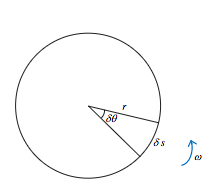
\includegraphics[scale=0.5]{img_M/13_intro1}
\end{center}

\subsection{Acceleration}
A particle moves in a circle of radius $r$ with constant speed , $v$.\\

Suppose that in a small time $\delta t$ the particle moves through a small angle $\delta\theta$, and that its velocity changes from $v_1$ to $v_2$, \\

then its change in velocity is $\delta v =v_2-v_1$, which is shown in the second diagram. \\

The lengths of both $v_1$ and $v_2$ are $v$, and the angle between $v_1$ and $v_2$ is $\delta\theta$.
\begin{align*}
	\delta v                  & = 2\times v \sin \frac{\delta\theta}{2}\approx 2v\times\frac{\delta\theta}{2}=v\delta\theta
	\frac{\delta v}{\delta t} & \approx v\frac{\delta\theta}{\delta t}
\end{align*}
as $\delta t \rightarrow 0 $, acceleration:
\[
	a=\frac{\d v}{\d t}=v\frac{\d \theta}{\d t}=v\theta
\]
But
\[
	\theta=\omega=\frac{v}{r} \rightarrow a = \frac{v^2}{r}=r\omega^2
\]
Notice that as $\delta\theta \rightarrow 0$, the direction of $\delta v$ becomes perpendicular to both $v_1$ and $v_2$, and so is directed towards the centre of the circle.\\

The acceleration of a particle moving in a circle with speed $v$ is $a=r\omega^2=\frac{v^2}{r}$, and is directed towards the centre of the circle.\\

Alternative proof
\begin{proof}
	If a particle moves , with constant speed, in a circle of radius $r$ and centre $O$, then its position vector can be written:
	\[
		\mathbf{r}=r\begin{pmatrix} \cos\theta \\ \sin\theta \end{pmatrix} \rightarrow \mathbf{\dot{r}}=r\begin{pmatrix}-\sin\theta \dot{\theta}\\ \cos\theta\dot{\theta}\end{pmatrix}
	\]
	Particle moves with constant speed $\rightarrow \dot{\theta}=\omega$ is constant
	\[
		\mathbf{\dot{r}}=r\begin{pmatrix}-\sin\theta \\ \cos\theta \end{pmatrix} \rightarrow v=r\omega
	\]
	\[
		\mathbf{\ddot{r}}=r\omega\begin{pmatrix}-\cos\theta \dot{\theta}\\ -\sin\theta\dot{\theta}\end{pmatrix}=-\omega^2r\begin{pmatrix} \cos\theta \\ \sin\theta \end{pmatrix}=-\omega^2\mathbf{r}
	\]
	acceleration is

	\[
		r\omega^2 \mbox{~or~} \frac{v^2}{r}
	\]
	directed towards $O$.
\end{proof}
\begin{center}
	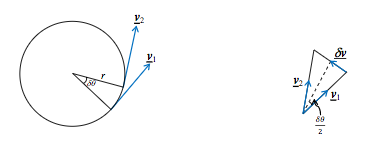
\includegraphics[scale=0.5]{img_M/13_intro2}
\end{center}

Types of problems:
\begin{enumerate}
	\item Horizontal
    \item Conical pendulum
    \begin{center}
        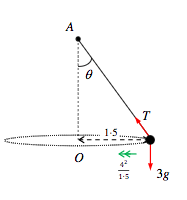
\includegraphics[scale=0.5]{img_M/13_eg1}
    \end{center}
	\item Banking
    \begin{center}
        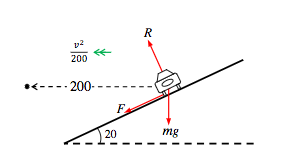
\includegraphics[scale=0.5]{img_M/13_eg2}
    \end{center}
	\item Inside an inverted vertical cone
    \begin{center}
        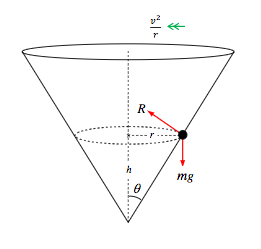
\includegraphics[scale=0.5]{img_M/13_eg3}
    \end{center}
\end{enumerate}

\subsection{Motion in a vertical circle}

\begin{prop}
	\[
		a=\frac{v^2}{r}
	\]
	\begin{proof}
		If a particle moves in a circle of radius $r$ and centre $O$, then its position vector can be written:
		\[
			\mathbf{r}=r\begin{pmatrix}\cos\theta\\ \sin\theta \end{pmatrix}
        \]
        \begin{align*}
        \mathbf{\dot{r}}&=r\begin{pmatrix}-\sin\theta \dot{\theta}\\ \cos\theta\dot{\theta}\end{pmatrix}=r\dot{\theta}\begin{pmatrix}-\sin\theta\\ \cos\theta \end{pmatrix}\\
        \mathbf{\ddot{r}}=r\begin{pmatrix}-\cos\theta\dot{\theta}^2-\sin\theta\ddot{\theta}\\-\sin\theta\dot{\theta}^2+\cos\theta\ddot{\theta}\end{pmatrix}=-r\dot{\theta}^2\begin{pmatrix}\cos\theta\\\sin\theta\end{pmatrix}+r\ddot{\theta}\begin{pmatrix}-\sin\theta\\\cos\theta\end{pmatrix}
        \end{align*}

        From this we can see that the speed is $v=r\dot{\theta}=r\omega$,\\
        and is perpendicular to the radius since $\mathbf{r\cdot\dot{r}}=0$\\
        
        We can also see that the acceleration has two components
        \[
            r\dot{\theta}^2=r\omega^2=\frac{v^2}{r}
        \]
        towards the centre opposite direction to $\mathbf{r}$\\
        
        and $r\ddot{\theta}$ perpendicular to the radius which is what we should expect since $v=r\dot{\theta}$ and $r$ is constant.\\
        
        In practice we shall onlu use 
        \[
            a=r\omega^2=\frac{v^2}{r}
        \]
        directed towards the centre of the circle
	\end{proof}
\end{prop}

Types of problems
\begin{enumerate}
    \item A particle attached to an inextensible string
    \begin{center}
        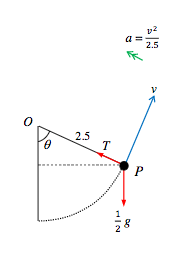
\includegraphics[scale=0.5]{img_M/13_eg4_1}
    \end{center}
    \begin{center}
        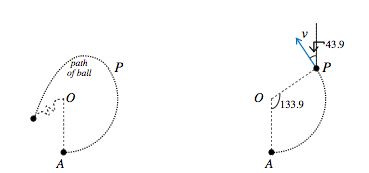
\includegraphics[scale=0.5]{img_M/13_eg4_2}
    \end{center}
	\item A particle moving on the indside of a smooth, hollow sphere
    \begin{center}
        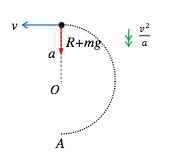
\includegraphics[scale=0.5]{img_M/13_eg5}
    \end{center}
	\item A particle attached to a rod
    \begin{center}
        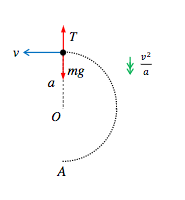
\includegraphics[scale=0.5]{img_M/13_eg6}
    \end{center}
	\item A particle moving on the outside of a smooth sphere
    \begin{center}
        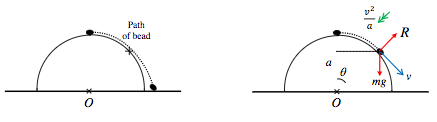
\includegraphics[scale=0.5]{img_M/13_eg7}
    \end{center}
\end{enumerate}
\section{Statics of rigid bodies 2}
\subsection{Centre of mass}
When finding a centre of mass \\

Centres of mass depend on the formula :
\[
    M\bar{x}=\sum m_ix_i
\]
or Similar, Remember that 
\[
    \lim_{\delta x\rightarrow 0}\sum f(x_i)\delta x=\int f(x) \d x
\]

\subsection{Centre of mass of geometric shapes}
\subsubsection{Sector}
In this case we can find a nice method, using the result for the centre of mass of a triangle.
\\
We take a sector of angle $2\alpha$ and divide it into many smaller sectors.\\

Mass of whole sector 
\[
    M=\frac{1}{2}r^2\times 2\alpha\times\rho=r^2\alpha\rho
\]
Consuder each small sector as approximately a triangle, with centre of mass, $G_1$, $2/3$ along the median from $O$\\

Working in polar coordinates for one small sector,
\[
    m_i=\frac{1}{2}r^2\rho\delta\theta
\]
\[
    OP=r\rightarrow OG_1 \cong \frac{2}{3}r \rightarrow x_i \cong \frac{2}{3}r\cos\theta 
\]
\begin{align*}
    \lim_{\delta\theta\rightarrow 0}\sum_{\theta=-\alpha}^{\alpha}m_ix_i&=\int_{-\alpha}^{\alpha}\frac{1}{2}r^2\rho\times \frac{2}{3}r\cos\theta\d\theta\\ 
    &=\frac{2}{3}r^3\rho\sin\alpha\\
    \bar{x}&=\frac{\sum m_ix_i}{M}=\frac{\frac{2}{3}r^3\rho\sin\alpha}{r^2\alpha\rho}=\frac{2r\sin\alpha}{3\alpha}
\end{align*}
By symmetry, $\bar{y}=0$\\
centre of mass is at $(\frac{2r\sin\alpha}{3\alpha},0)$
\begin{center}
    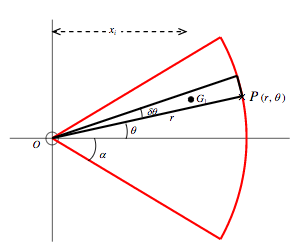
\includegraphics[scale=0.5]{img_M/14_intro1}
\end{center}
\subsubsection{Circular arc}
For a circular arc of radius $r$ which subtends an angle of $2\alpha$ at the centre. \\

The length of the arc is $r\times 2\alpha$ \\
The mass of the arc is $M=2\alpha r \rho$ \\

First divide the arc into several small pieces, each subtending an angle of $\delta\theta$ at the centre \\

The length of each piece is $r\delta\theta\rightarrow m_i=r\rho\delta\theta$\\

We now think of each small arc as a point mass at the centre of the arc, with $x$-corrdinate $x_i=r\cos\theta$\\

\begin{align*}
    \lim_{\delta\theta\rightarrow0}\sum_{\theta=-\alpha}^{\alpha}m_ix_i&=\int_{-\alpha}^{\alpha}r\rho\times r \cos\theta\d\theta \\
    &= 2r^2\rho\sin\alpha \\
    \bar{x}&=\frac{\sum m_ix_i}{M}=\frac{2r^2\rho\sin\alpha}{2r\alpha\rho}=\frac{r\sin\alpha}{\alpha}
\end{align*}
By symmetry, $\bar{y}=0$\\
centre of mass is at $(\frac{r\sin\alpha}{\alpha},0)$
\begin{center}
    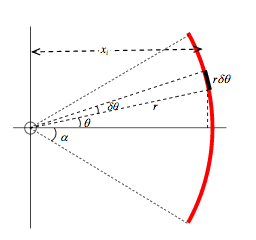
\includegraphics[scale=0.5]{img_M/14_intro2}
\end{center}

\subsubsection{Others}
\begin{center}
    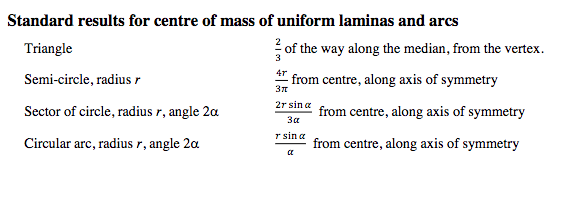
\includegraphics[scale=0.5]{img_M/14_others}
\end{center}

\subsubsection{Solid of revolution}
\begin{center}
    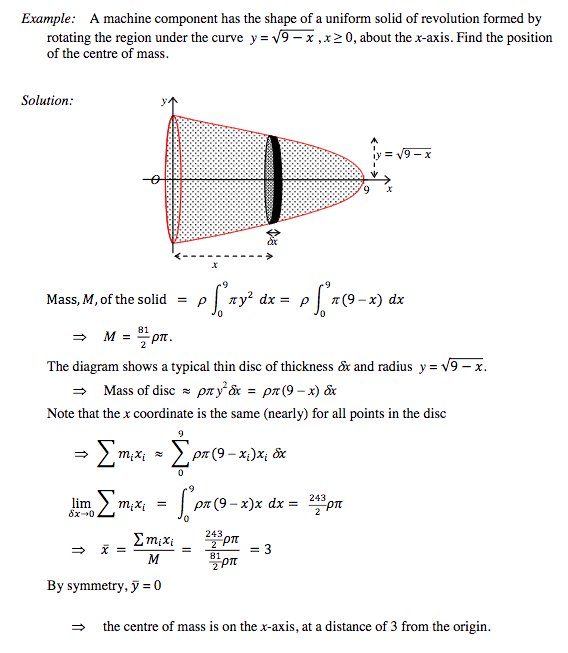
\includegraphics[scale=0.5]{img_M/14_eg1}
\end{center}
\subsubsection{Hemispherical shell}
\begin{center}
    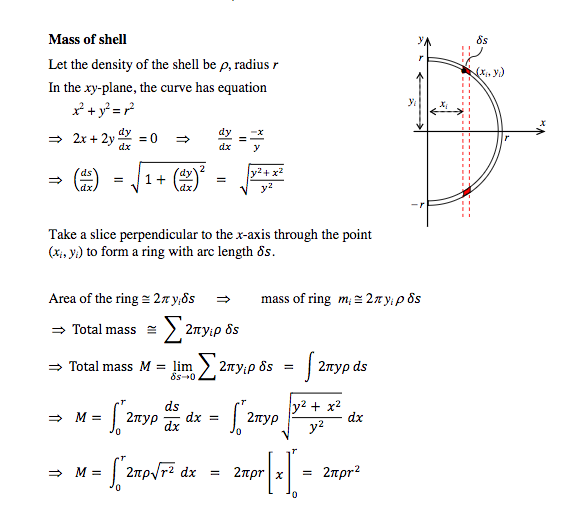
\includegraphics[scale=0.5]{img_M/14_eg2}
\end{center}
\begin{center}
    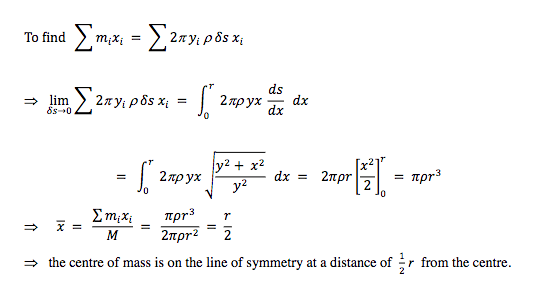
\includegraphics[scale=0.5]{img_M/14_eg2_2}
\end{center}
\begin{center}
    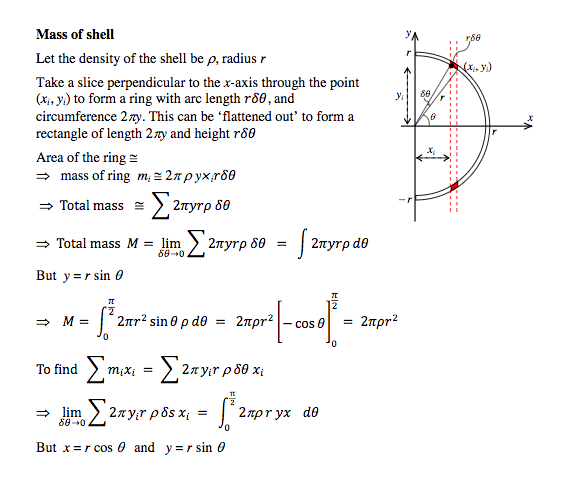
\includegraphics[scale=0.5]{img_M/14_eg2_3}
\end{center}
\begin{center}
    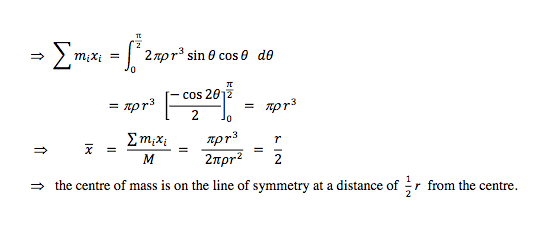
\includegraphics[scale=0.5]{img_M/14_eg2_4}
\end{center}
\subsubsection{conical}
\begin{center}
    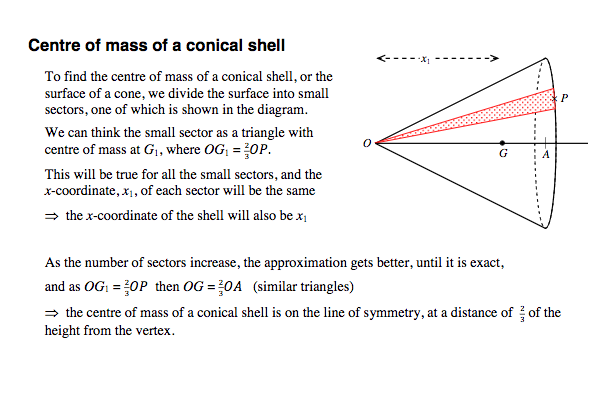
\includegraphics[scale=0.5]{img_M/14_intro3}
\end{center}
\subsubsection{Square based pyramid}
\begin{center}
    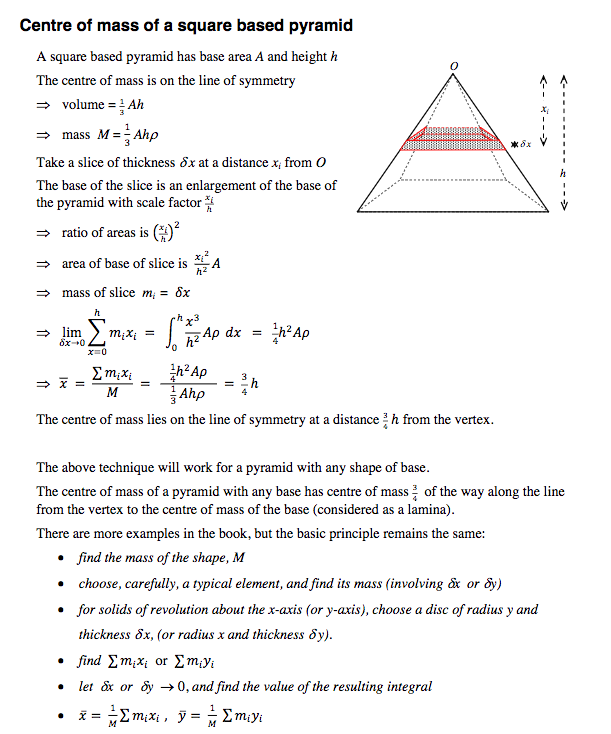
\includegraphics[scale=0.5]{img_M/14_intro4}
\end{center}
\subsubsection{The standard results}
\begin{center}
    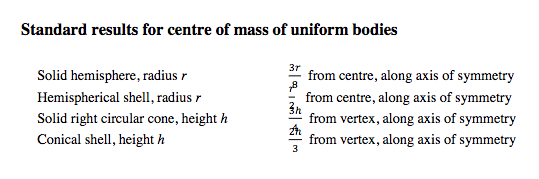
\includegraphics[scale=0.5]{img_M/14_intro5}
\end{center}
\begin{center}
    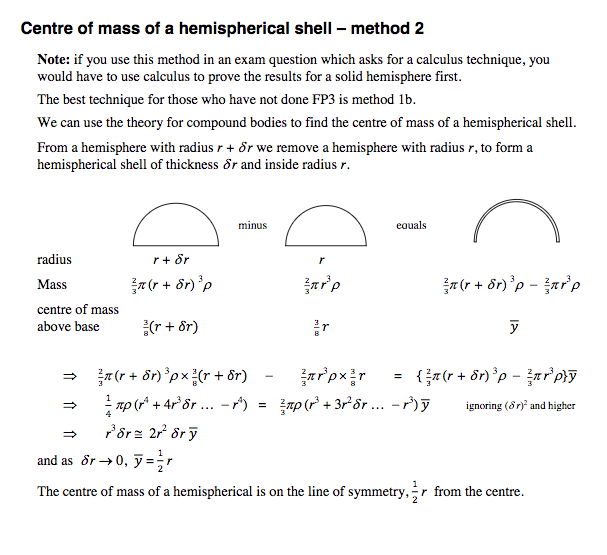
\includegraphics[scale=0.5]{img_M/14_intro6}
\end{center}

\subsubsection{Tilting and hanging freely}

\begin{center}
    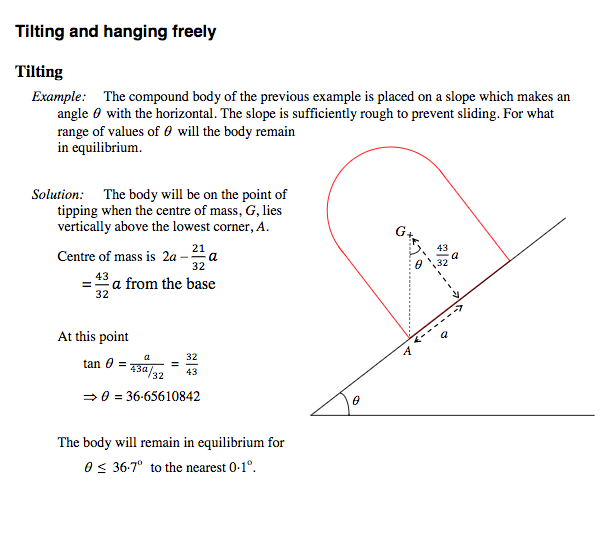
\includegraphics[scale=0.5]{img_M/14_intro7}
\end{center}
\begin{center}
    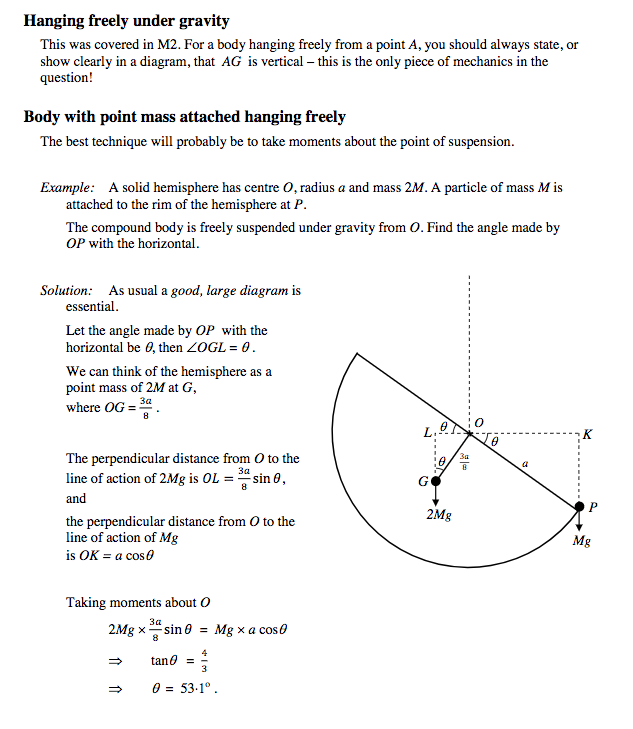
\includegraphics[scale=0.5]{img_M/14_eg3}
\end{center}

\subsubsection{Hemisphere in equilibrium on a slope}
\begin{center}
    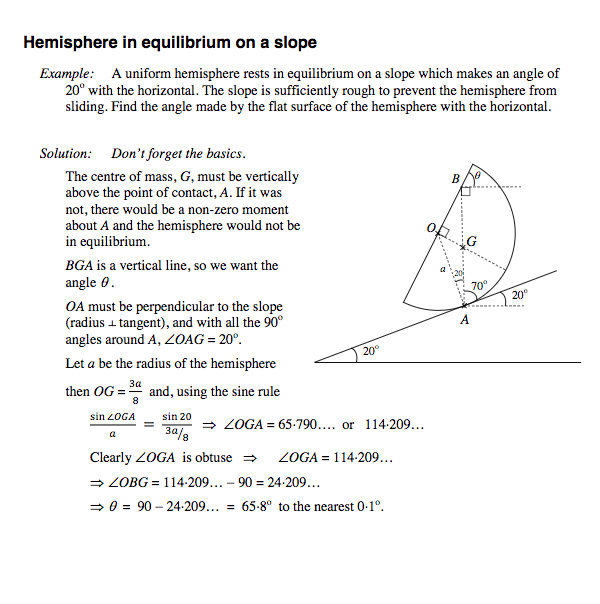
\includegraphics[scale=0.5]{img_M/14_eg4}
\end{center}

\section{Relative motion}

\section{Elastic collisions in two dimensions}

\section{Resisted motion of a particle moving in a straight line}

\section{Damped and forced harmonic motion}

\section{Stability}

\section{Applications of vectors in mechanics}

\section{Variable mass}

\section{Moments of inertia of a rigid body}

\section{Rotation of a rigid body about a fixed smooth axis}




\printindex



\end{document}}